\documentclass[a4paper, 12pt]{scrartcl}
\usepackage[utf8]{inputenc}
\usepackage[ngermanb]{babel}
\usepackage{setspace}
\usepackage{geometry}
\usepackage{graphicx}
\usepackage{cite}
\usepackage{amsmath}
\geometry{a4paper, top=25mm, left=25mm, right=25mm, bottom=25mm}

\title{Seminar IT-Sicherheit}
\author{Kevin Seidel \\ Studiengang Informatik \\ Matrikelnummer: 943147}

\begin{document}
\begin{titlepage}
\begin{center}
\vspace*{1.5cm}
\begin{Large}
\textbf{Universität Osnabrück}
\end{Large}

\noindent\hrulefill
\\[3.5cm]
PRAKTIKUMSBERICHT \\[1cm]
zum Programmierpraktikum \\[1cm]
\textbf{Paralelle Algorithmen mit OpenCL} \\[1.5cm]
im Sommersemester 2013 \\[1.5cm]
Thema: \\[0.5cm]
\textbf{Voxelization} \\[2cm]
Erstellt am 15.10.2013
\end{center}
\vfill
\begin{flushleft}
Vorgelegt von: 
\hfill \parbox{46mm}{Kevin Seidel} \\
\hfill \parbox{46mm}{943147} \\
\hfill \parbox{46mm}{Falkenstra"se 43} \\
\hfill \parbox{46mm}{49124 Georgsmarienh"utte}
\end{flushleft}
\end{titlepage}

\newpage

\pagenumbering{Roman}
\setcounter{page}{2}
\tableofcontents

\newpage
\pagenumbering{arabic}
\setcounter{page}{1}

\section{Einleitung}
W"ahrend des Praktikums habe ich mich mit der Voxelization von Szenen auf der GPU besch"aftigt. Dabei geht es darum, eine aus Polygonen bestehende Szene in eine Voxelgatter zu "uberf"uhren. Um diese Aufgabe in Echtzeit auszuf"uhren wird daf"ur die Grafikkarte genutzt, da diese, auf Grund ihrer hohen Paralellit"at, sehr gut daf"ur geeignet ist.
Die gewonnenen Voxeldaten k"onnen danach f"ur das Beleuchtungsmodell verwendet werden. Dadurch ist es beispielsweise m"oglich die indirekte Beleuchtung oder die Ambient Occlusion einer Szene in Echtzeit zu berechnen.
Im weiteren Verlauf dieses Berichts wird auf zwei verschiedene M"oglichkeiten der Voxelizierung eingegangen. Ausserdem wird noch ein effizentes Speichermodell der Voxeldaten, der sogenannt Sparse Voxel Octree gezeigt, welcher sowohl eine kompakte Speicherung der Daten als auch einen schnellen Zugriff auf die gespeicherten Voxel erlaubt. 
Abschlie"send wird noch auf die weitere Nutzung der erzeugten Voxeldaten eingegangen, speziell auf die indirekte Beleuchtung der Szene.

\section{Voxel und Voxelization}
\subsection{Voxel}
Das Wort Voxel setzt sich aus den englischen Begriffen ''volumetric'' und ''pixel'' zusammen. Frei "ubersetzt kann man es als einen dreidimensionalen Pixel bezeichnen.
Das Voxel hat im Allgemeinen nur zwei Eigenschaften, welche dem eines Pixels gleichkommen. Es besitzt eine Position in einem vorher festgelegtem, dreidimensionalen Raum und einen Farbwert.
Dieser 3D-Raum ist dabei in, in jeder Richtung, gleichgro"se Voxel unterteilt.
F"ur meinen Verwendungszweck wird das Voxel als W"urfel dargestellt, wobei alle Seiten die Farbe des Voxels tragen.
\subsection{Voxelization}
Die Voxelization ist die "Uberf"uhrung einer Szene aus Polygonen in ein Voxelgitter, wobei f"ur jedes Voxel bestimmt wird, ob es ein Polygon "uberschneidet oder nicht.

Bei der Voxelization gibt es verschiedene Verfahren. Zum einen die Oberfl"achen-Voxelization,  welche nur direkte "Uberschneidung der Polygone mit Voxeln im Gitter erfasst. Es wird also nur die Oberfl"ache der Polygone ber"ucksichtigt.

Eine andere Methode ist die solide Voxelization, welche testet, ob ein Voxel innerhalb eines Objekts liegt. Dadurch werden Modelle innerhalb der Szene komplett ausgef"ullt, was man ich Abbildung 1 sehr gut erkennen kann.

\begin{figure}[h]
	\centering
		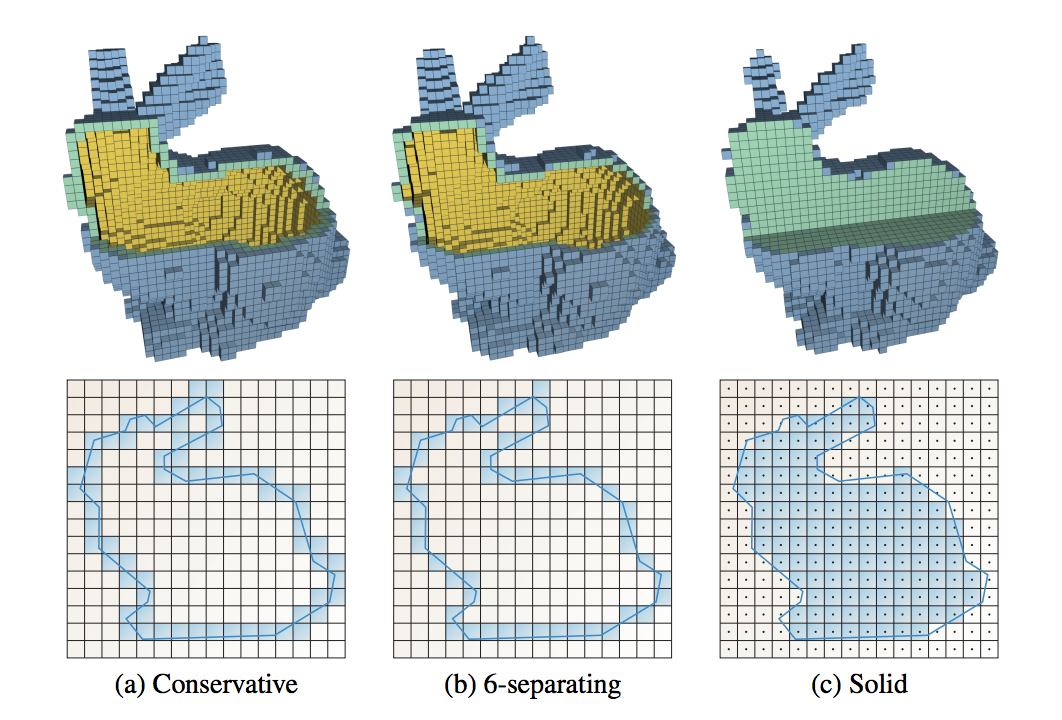
\includegraphics[width=14cm]{Kinds-of-Voxelization}
	\caption{Verschiedene Arten der Voxelization}
\end{figure}

F"ur die Nutzung der Voxel zur Beleuchtung reicht jedoch eine Oberfl"achen-Voxelization aus, so dass im weiteren Verlauf nur darauf eingegangen wird.

Diese Aufgabe kann hochgradig paralell ausgef"uhrt werden, wodurch sich die Nutzung der GPU f"ur dieses Verfahren anbietet. In der Literatur zu diesem Problem gibt es mehrere L"osungsans"atze. 
In fr"uheren Arbeiten wurde die Szene in mehrere Ebenen, entsprecht der Gr"o"se des Voxelgitters, eingeteilt, sodass jede Voxelebene seperat gerendert wurde. Dies f"uhrt dazu, dass diese Verfahren sehr langsam ist, da f"ur h"ohere Dimensionen sehr viele Renderaufrufe durchgef"uhrt werden m"ussen.

Eine etwa neuere Taktik nutzt die Paralellisierbarkeit dieser Aufgabe aus und "uberpr"uft Kollisionen zwischen den Polygonen und den Voxeln mittels GPU-Computing. Dieser Ansatz kann sowohl mittels Cuda als auch mittels OpenCL gel"ost werden.
Bei dieser neueren Methode wird f"ur jedes Polygon in der Szene ein eigener Thread gestartet und innerhalb dieses Threads wird "uberpr"uft, ob das Polygon ein Voxel "uberschneidet. Das Ergebnis wird dann in einen Buffer geschrieben, welcher dann f"ur jede Stelle des Voxelgrids einen Wert enth"alt, welcher angibt, ob das Voxel gef"ullt ist oder nicht.

Ein weiterer, neuerer Ansatz nutzt f"ur die Bestimmung der Voxel die feste OpenGL-Pipeline, im genaueren den Hardware-Rasterizer. Dies erm"oglicht eine noch k"urzere Laufzeit, bringt jedoch auch einige Probleme mit sich.

Die beiden Ans"atze mittels OpenGL und OpenCL werden in weiteren Verlauf genauer erl"autert.



\section{Voxelization mit Hilfe von OpenGL}
Zuerst habe ich mich mit der Voxelization mittels OpenGL besch"aftigt. Dieser Ansatz ist eine neuere Methode, da hierbei Funktionen aus OpenGL 4.2 genutzt werden. Diese Version erschien im August 2011. 
Der OpenGL-Ansatz nutzt hierbei die feste Hardware-Pipleline der Grafikkarte aus, um den Prozess der Voxelization zu beschleunigen. 
Der Vorteil dieser Methode ist, dass sie nur einen einzigen Render-Durchlauf ben"otigt.
Hierbei wird im spezifischen der Hardware-Rasterizer genutzt, um die "Uberschneidung der Polygone und der Voxel zu bestimmen. 

Ein Problem, welches hierbei auftaucht, ist, dass der Rasterizer dar"ur gedacht ist, eine zwei-dimensionale Szene zu rastern. F"ur das hier vorliegende Problem muss jedoch eine dreidimensionale Szene gerastert beziehungsweise voxelisiert werden.

Um dieses Problem zu l"osen, wird das Polygon, mittels Paralellprojektion, auf eine zweidimensionale Ebene projeziert.
Die Zielebene wird so gew"ahlt, dass das Polygon die gr"o"st m"ogliche Fl"ache auf dieser Ebene einnimmt.
Im dreidimensionalen Raum kommen daf"ur drei Ebenen in Frage. 
Um die geeignete Ebene zu finden, bestimmt man die dominante Achse der Normalen. 
Die dominanten Achse ist die, in welche der Normalenvektor die h"ochste Ausdehnung aufwei"st.
Ist beispielsweise die dominanten Achse die x-Achse, w"are die zu w"ahlende Ebene, die yz-Ebene.

Diese Projektion auf eine 2D-Ebene geschieht individuell f"ur jedes Polygon im Geometry-Shader des jeweiligen Renderaufrufs.
Hierdurch wird die gr"o"st m"ogliche Fl"ache des Dreiecks rasterisiert, wodurch m"ogliche L"ucken in der Voxelization reduziert werden. Durch die Rasterisierung erh"alt man die Pixel, welche vom Polygon "uberlappt werden. Um diese zweidimensionalen Positionsinformationen nun in Voxel zu "uberf"uhren, werden die Pixel nun entgegen der zuvor bestimmten dominanten Achse, zur"uck projeziert, sodass sich die Positioninformation nun im dreidimensionalen Raum befinden. Dadurch erh"alt man die Position der Voxel.

\begin{figure}[h]
	\centering
		\includegraphics[width=16cm]{Voxelization-Pipeline}
	\caption{Schritte der Voxelization mittels OpenGL}
\end{figure}

Die entstehenden Voxel werden dann mittels der in OpenGL 4.2 eingef"uhrten Methode ''image store'', welche es erlaubt, im Fragment-Shader, an eine beliebige Stelle in einer Textur zu schreiben, in eine 3D-Textur geschrieben. Hierbei wird die Position des Voxels und dessen Farbwert geschrieben.


Mittels dieser Textur lassen sich die Voxel nun problemlos ausgeben. Es ist also m"oglich zu "uberpr"ufen, ob ein Voxel vorhanden ist und welche Farbe er besitzt.

Eine Schw"ache dieser Methode ist, dass es vorkommen kann, dass auf Grund der n"otigen Projektion einige Voxel nicht registriert werden. Dies ist darauf zur"uckzuf"uhren, dass "Uberschneidungen nur am Mittelpunkt des Pixel getestet werden. Hierf"ur existiert jedoch eine L"osung: 

Das zu testende Polygon wird so vergr"o"sert, dass das vorherige Polygon, welches einen Pixel nur ber"uhren w"urde, nun den Mittelpunkt "uberschneidet. 

\newpage

\section{Voxelization mit Hilfe von OpenCL}
Bei der Voxelization mittels OpenCL muss die Erkennung von "Uberschneidungen individuell programmiert werden, da hier nicht auf einen feste Pipeline zur"uckgegriffen werden kann. Dies erlaubt jedoch auch mehr Freiheiten bei der Erkennung, Verarbeitung und Speicherung der Voxeldaten. 

Bei der "Uberf"uhrung von Polygonen in Voxel mittels eines OpenCL-Kernels wird f"ur jedes Polygon der zu voxelisierenden Szene ein eigener Thread gestartet, sodass alles Polygone paralell bearbeitet werden. 
In jedem Kernelaufruf wird daf"ur auf die "Uberschneidung zwischen dem jeweiligen Polygon und den Voxeln getestet. Um diesen Vorgang zu beschleunigen, wird nur in der in Frage kommenden Bounding-Box des aktuellen Dreiecks auf "Uberschneidungen getestet.

Das hei"st, es werden zuerst die Eckpunkte einer Box berechnet, welche das Dreieck genau umschlie"sen w"urde. Dadurch muss nicht die komplette Szene auf "Uberschneidungen getestet werden, sondern nur ein kleinerer Ausschnitt.

F"ur jedes Voxel ,innerhalb dieser Box, wird nun getestet, ob sich ein oder mehrere Eckpunkte des Voxels auf verschiedenen Seiten eines Polygons befinden. Dadurch werden die Voxel bestimmt, welche sich an den Seiten oder Ecken des Polygons befinden.


Des Weiteren wird "uberpr"uft, ob sich die 2D-Projektion des Polygons und des Voxels "uberlappen. 

Wenn beide Tests eine "Uberschneidung best"atigen, ist eine "Uberschneidung best"atigt und kann so geschrieben werden.
Die Speicherung der Voxel ist bei diesem OpenCL Ansatz frei w"ahlbar. 
In meinem Ansatz wurden alle Voxel in einen eindimensionalen Buffer geschrieben. 

\begin{figure}
		$Buffer: (x0, y0, z0), (x0, y0, z1), ..., (x0, y0, z511), (x0, y1, z0), ..., (x511, y511, z511)$
\caption{Aufbau des Buffers f"ur ein Voxelgrid der Dimension $512^3$}

\end{figure}

Es w"are auf Grund der Freiheit, welche man durch die Verwendung eines eigenen OpenCL-Kernels zur Verf"ugung hat, jedoch auch m"oglich die Voxeldaten direkt in einen Sparse Voxel Octree zu schreiben, wodurch keine weitere Umwandlung der Datenstruktur mehr n"otig ist, da der Sparse Voxel Octree schon die gewollte Speicherart ist.

\section{Vergleich zwischen OpenGL und OpenCL Ansatz}
Wie bereits erw"ahnt, liegt der Hauptunterschied beider Varianten an der Nutzung der festen Hardware der Grafikkarte. 
Der Ansatz mittels OpenGL erlaubt, auf Grund der Nutzung dieser festen Hardware eine schnellere Ausf"uhrung der Voxelization.
Dies ist besonders im Bezug auf die Nutzung von schw"acherer Hardware, zum Beispiel auf mobilen Ger"aten, zu bevorzugen, jedoch auch auf performanter Hardware ein guter Ansatz.

Der Vorteil der OpenCL-Variante ist die gr"o"sere Freiheit bei der Voxelization, da man seinen OpenCL-Kernel nach eigenen Vorstellungen erstellen kann.
So l"asst sich eineigener Kernel mit individueller Voxelerkennung, Datenverarbeitung und Datenspeicherung erstellen. 
Somit ist es m"oglich die Voxelization komplett nach den eigenen Bed"urfnissen anzupassen, wobei man jedoch immer die Performanz ber"ucksichtigen sollte, welche bei sehr komplexen Kerneln leiden k"onnte.



\section{Speicherung der Voxeldaten}
Um die Nutzung zu beschleunigen und den Speicherbedarf gering zu halten, werden die Voxel in sogenannten Sparse Voxel Octrees gespeichert. 
Ein Octree ist eine Baumstruktur, wobei jeder Knoten jeweils acht Kindknoten hat. Diese Struktur ist sehr geeignet, da bei der Aufteilung eines W"urfels in gleichm"a"sige St"ucke, acht neue W"urfel entstehen.

Ein weiterer Vorteil der Sparse Voxel Octrees ist, dass der entstehende Baum nicht gleichm"a"sig aufgebaut sein muss. 
Das hei"st, dass jeder Teilbaum eine beliebige Tiefe aufweisen kann.
So lassen sich zusammenh"angende Voxel des gleichen Typ (z.B. Farbe) zusammenfassen und der Baum muss nicht weiter in die Tiefe wachsen.
Diese Methode spart zum einen Speicherplatz, da nicht zwingend f"ur jedes Voxel ein Wert vorgehalten werden muss, sondern beschleunigt auch die weitere Verarbeitung, auf Grund der schnelleren "Uberpr"ufung der Voxeldaten.

\section{Nutzung der Voxeldaten}
Nachdem diese Voxeldaten erzeugt wurden, stellt sich nun die Frage, wie diese weiterverarbeitet werden.
Die Voxel beziehungsweise das entstandene Voxelgrid sollte in diesem Fall f"ur ein Beleuchtungsmodell verwendet werden. Im Genaueren sollte mittels der Voxeldaten die indirekte Beleuchtung errechnet werden.

Dabei wird das sogenannte Voxel Cone Tracing verwendet, welches einem vereinfachten und simplerem Raytracing entspricht.

Hierbei wird nicht , wie beim klassischen Raytracing, f"ur jeden Bildpunkt ein Strahl in die Szene geschossen, sondern ein Kegel, welcher in naher Distanz relativ hochaufl"osend ist, f"ur weiter entfernte Berechnungen jedoch nur eine N"aherung liefert, wie auch in Abbildung 4 zu sehen.
Das hei"st, im Bezug auf die Speicherung der Daten in einem Sparse Voxel Octree, das f"ur Nahe Objekte sehr tief in den Octree geschaut wird, f"ur die entfernten Objekte jedoch nur oberen Ebenen des Baumes betrachtet werden.
Durch die Nutzung des Octrees und des Voxel Cone Tracing, ist diese Methode bedeutend schneller als das klassischen Raytracing, da deutlich weniger Daten verarbeitet werden m"ussen.

\begin{figure}[h]
	\centering
		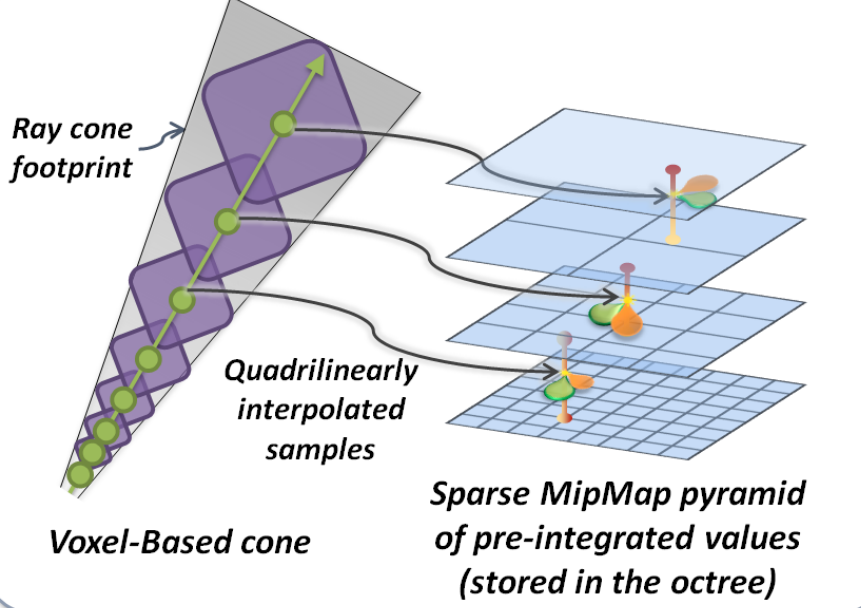
\includegraphics[width=12cm]{voxel-cone-tracing}
	\caption{Voxel Cone Tracing}
\end{figure}

\newpage

\section{Ausblick und Fazit}
Mit heutiger Hardware ist ein Echtzeit-Raytracing einer komplexen Szene und zu einer brauchbaren Bildrate noch nicht m"oglich. Die von mir vorgestellte Methode, bestehend aus Voxelization, der Sparse Voxel Octree-Speicherung und des Voxel Cone Tracing, k"onnen auf heutiger Hardware schon zufriedenstellende Beleuchtungsergebnisse und Bildraten erzielen. 
Daher ist dieser Ansatz f"ur die n"ahere Zukunft sehr vielversprechend, da auch bei steigenden Aufl"osungen der Szenen noch zufriedenstellende Ergebnisse erzielt werden k"onnen, wohingegen das Raytracing mit der heute zug"anglichen und auch zuk"unftigen Hardware noch einige Jahre brauchen wird, bis es f"ur die Echtzeitdarstellung von 3D-Szenen genutzt werden kann, da hierf"ur eine deutlich schnellere Grafikhardware von N"oten ist.

\end{document}